% teil0.tex -- Einleitung
%
% Motivation: Wir können den Fundamentalsatz, aber wir wissen nicht,
% wo die Nullstellen sind. Bisektion auf R als Brücke zur Idee in C.
%
% (c) 2026 Lukas Krüdewagen, OST Ostschweizer Fachhochschule
%
% !TEX root = ../../buch.tex
% !TEX encoding = UTF-8
%
\section{Einleitung%
\label{weyl:section:einleitung}}
\kopfrechts{Einleitung}
Der Fundamentalsatz der Algebra sichert uns zu, dass jedes komplexe Polynom
\[
f(z)
=
a_n z^n + a_{n-1} z^{n-1} + \dots + a_1 z + a_0
\]
vom Grad $n \geq 1$ genau $n$ Nullstellen in $\mathbb{C}$ besitzt, mit Vielfachheit
gezählt.
Der Satz garantiert allerdings nur die Existenz, er sagt uns nichts darüber, \emph{wo}
diese Nullstellen liegen.
Hermann Weyl bemerkte dazu treffend, der Fundamentalsatz verkünde
\index{Weyl, Hermann}
"`das Vorhandensein eines Schatzes, ohne jedoch zu verraten, an welchem Ort"'
\cite{weyl:eisermann}.

Für Grad $n = 1$ und $n = 2$ kennen wir explizite Lösungsformeln, für $n = 3$ und
$n = 4$ existieren noch die Formeln von Cardano und Ferrari.
\index{Cardano, Gerolamo}%
\index{Ferrari, Lodovico}%
Ab $n \geq 5$ jedoch gibt es nach Abel und Galois keine allgemeine Wurzelformel mehr.
\index{Abel, Niels Henrik}%
\index{Galois, Evariste@Galois, Évariste}%
In der Praxis muss man sich daher mit numerischen Methoden begnügen, die die Nullstellen
\emph{lokalisieren} und \emph{approximieren}.

Das wohl bekannteste solche Verfahren ist das Newton-Verfahren.
\index{Newton-Verfahren}%
Es konvergiert in der Nähe einer Nullstelle quadratisch und damit sehr schnell, hat aber
\index{Konvergenz!quadratisch}%
einen empfindlichen Schwachpunkt: man muss einen ausreichend guten Startwert kennen.
\index{Startwert}%
Wählt man den Startwert ungeschickt, kann das Verfahren divergieren, in einen Zyklus
geraten oder gegen eine andere als die gesuchte Nullstelle konvergieren.
Diese Schwachstelle wird in Abschnitt~\ref{julia:zweck} des Kapitels über Julia-Mengen
\index{Julia-Menge}%
genauer erläutert.
Bei einem Polynom vom Grad $n$ mit $n$ verschiedenen Nullstellen reicht es zudem nicht,
nur \emph{eine} Nullstelle zu finden, man möchte sie alle bestimmen und zwar
zuverlässig.

\subsection{Idee aus dem Reellen: Bisektion%
\label{weyl:subsection:bisektion}}
\index{Bisektion}%
Für reelle stetige Funktionen $g\colon [a,b] \to \mathbb{R}$ liefert der Zwischenwertsatz
ein einfaches und global zuverlässiges Verfahren: gilt $g(a) \cdot g(b) < 0$, so liegt
zwischen $a$ und $b$ mindestens eine Nullstelle.
Man halbiert das Intervall, prüft in welcher Hälfte das Vorzeichen wechselt, verwirft
die andere Hälfte und wiederholt das Spiel.
Die Idee ist robust, einfach und garantiert konvergent, nur eben langsam, denn die
Genauigkeit verdoppelt sich pro Schritt nur um ein Bit.
In Abbildung~\ref{weyl:fig:bisektion} ist das Prinzip skizziert.

%
% fig/bisektion.tex -- Bisektion auf R
%
\begin{figure}
\centering
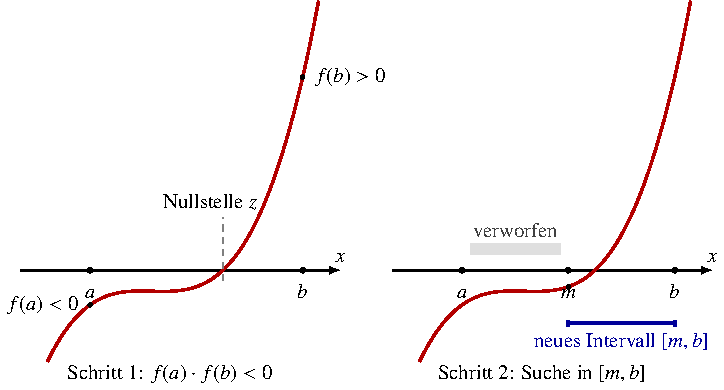
\includegraphics{papers/weyl/images/bisektion.pdf}
\caption{Bisektion einer reellen stetigen Funktion: das Vorzeichen wechselt
zwischen $a$ und $b$, also liegt nach dem Zwischenwertsatz mindestens eine
Nullstelle dazwischen. Durch Halbieren und Auswählen der Hälfte mit
Vorzeichenwechsel verkleinert sich der Suchbereich pro Schritt um den Faktor zwei.
\label{weyl:fig:bisektion}}
\end{figure}


Möchte man diese Idee in die komplexe Ebene übertragen, stösst man sofort auf ein
Problem: in $\mathbb{C}$ gibt es kein Vorzeichen.
Der Zwischenwertsatz greift nicht, denn ein komplexer Funktionswert hat keine zwei
\index{Zwischenwertsatz}%
``Seiten'', zwischen denen ein Wechsel stattfinden könnte.
Wir brauchen also einen Ersatz: einen Test, der uns für ein zweidimensionales Gebiet
$D \subseteq \mathbb{C}$ verrät, ob darin Nullstellen liegen und im Idealfall
gleich auch wie viele.

Genau dies leistet \emph{Weyls Quadtree-Algorithmus}, den Hermann Weyl 1924 in
\cite{weyl:weyl1924} vorgeschlagen hat.
\index{Quadtree-Algorithmus}%
Er übersetzt das Bisektionsprinzip von eindimensionalen Intervallen auf
zweidimensionale Quadrate.
Statt eines Vorzeichenwechsels nutzt er ein \emph{Wegintegral}: Nach dem
Argumentprinzip zählt das Integral von \(f'/f\) entlang des Randes eines Gebiets die
\index{Argumentprinzip}%
Anzahl der darin liegenden Nullstellen abzüglich der Polstellen, jeweils mit
Vielfachheit, ohne dass man deren Lage vorher kennen müsste.
Anschliessend wird das Verfahren mit dem Newton-Verfahren kombiniert. Der Quadtree
liefert die grobe Lokalisation und garantiert, alle Nullstellen zu finden, das
Newton-Verfahren übernimmt die schnelle Feinkonvergenz.

\subsection{Aufbau dieses Kapitels%
\label{weyl:subsection:aufbau}}
Das Kapitel ist wie folgt aufgebaut.
In Abschnitt~\ref{weyl:section:grundlagen} stellen wir die Werkzeuge aus der komplexen
Analysis zusammen, auf die der Algorithmus aufbaut: das Wegintegral, den Cauchy-Integralsatz und das Argumentprinzip.
Da diese Grundlagen bereits in den vorangehenden Kapiteln des Buches eingeführt wurden,
beschränken wir uns auf das Wesentliche und zeigen vor allem, \emph{wie} sie in
Weyls Algorithmus zusammenwirken.
Abschnitt~\ref{weyl:section:algorithmus} beschreibt den Quadtree-Algorithmus
selbst, Schritt für Schritt und mit einem ausgearbeiteten Beispiel.
Abschnitt~\ref{weyl:section:hybrid} schliesslich erläutert die Kombination mit dem
Newton-Verfahren und ordnet das Verfahren in die heutige Landschaft der
Nullstellensucher ein.
\index{Nullstellensucher}%

